\documentclass[a4paper, utf8]{article}
\author{Kim Rune Solstad}
\title{Assignment 1, TDT4205}
\usepackage{listings, tikz}
\usepackage[utf8]{inputenc}
\usetikzlibrary{automata, positioning}

\lstset{language=bash}

\begin{document}
\maketitle
\section*{Part 1, Theory}
\subsection*{Problem 1}
Login gikk greit ved å bruke

\begin{lstlisting}
ssh kmirs@stud.ntnu.no
\end{lstlisting}

Version til gcc er 4.6.3. Version til flex er 2.5.35. Version til bison er 2.5. Fant disse ved å bruke 
\begin{lstlisting}
gcc --version
flex --version
bison --version
\end{lstlisting}

\subsection*{Problem 2}
Interpreter: Kjører programkode uten å oversette sammen med input fra bruker for å returnere et svar.
Kompilator: Oversetter programkoden til maskinkode som kan kjøres. 

\subsection*{Problem 3}
\emph{a)} \\
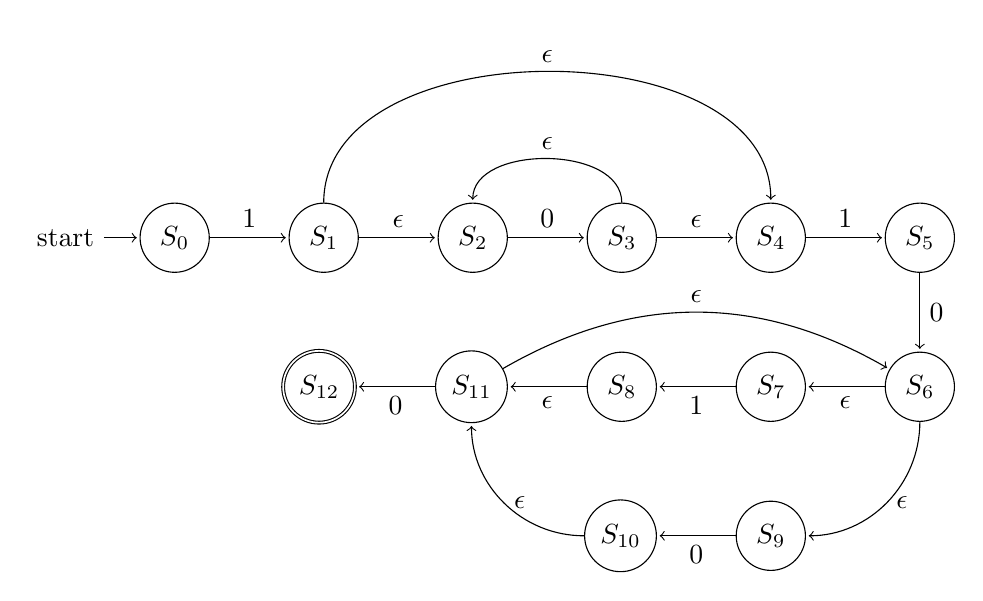
\begin{tikzpicture}[->, shorten >=1pt, auto]
	\node[state,initial] 	(A)   						{$S_0$}; 
	\node[state] 			(B) [right			=of A] 	{$S_1$}; 
	\node[state] 			(C) [right			=of B] 	{$S_2$};	
	\node[state] 			(D) [right			=of C] 	{$S_3$};
	\node[state] 			(E) [right			=of D] 	{$S_4$};
	\node[state] 			(F) [right			=of E] 	{$S_5$};
	
	\node[state] 			(G) [below 			=of F] 	{$S_6$};
	\node[state] 			(H) [below, left 	=of G] 	{$S_7$};
	\node[state] 			(I) [left			=of H] 	{$S_8$};	
	\node[state] 			(J) [below			=of H] 	{$S_9$};
	\node[state] 			(K) [left			=of J] 	{$S_{10}$};
	\node[state] 			(L) [left			=of I] 	{$S_{11}$};
	\node[state, accepting] (M) [left			=of L] 	{$S_{12}$};

	\path[->]
	(A) edge 						node 	{1}				(B)
	(B) edge [in=90, out=90, above] node	{$\epsilon$}	(E)
		edge						node	{$\epsilon$}	(C)
	(C)	edge						node	{0} 			(D)
	(D)	edge						node	{$\epsilon$}	(E)
		edge [in=90, out=90, above] node	{$\epsilon$}	(C)
	(E)	edge						node	{1}				(F)
	(F) edge [in=90, out=-90,right]	node	{0}				(G)
	(G)	edge 						node	{$\epsilon$}	(H)
		edge [in=0,out=-90,  right]	node	{$\epsilon$}	(J)
 	(H) edge						node	{1}				(I)
	(I)	edge						node	{$\epsilon$}	(L)
	(J) edge						node	{0}				(K)
	(K)	edge [in=-90,out=180, right]node	{$\epsilon$}	(L)
	(L) edge [in=150, out=30, above]node	{$\epsilon$}	(G)	
		edge						node	{0}				(M)
;

	
\end{tikzpicture}
\\
%\begin{tikzpicture}[->, shorten >=1pt, auto]
%	\node[state]	(G)	{$S_6};
%\end{tikzpicture}


\emph{b)}
Alle ord som begynner på 1 etterfulgt av ingen eller flere 0 etterfulgt av 1 etterfulgt av 0 etterfulgt av en ubegrenset kombinasjon av 0 og 1 avsluttet med 0. \\

\emph{c)}	\\

\begin{tabular}{c | c c c}
state 	& 1				& 0				& $\epsilon$	\\
\hline
0 		& 1			 	& $\emptyset$ 	& $\emptyset$	\\
1 		& $\emptyset$ 	& $\emptyset$ 	& 2, 4			\\
2 		& $\emptyset$ 	& 3			 	& $\emptyset$	\\
3 		& $\emptyset$ 	& $\emptyset$ 	& 2, 4			\\
4 		& 5			 	& $\emptyset$ 	& $\emptyset$	\\
5 		& $\emptyset$ 	& 6			 	& $\emptyset$	\\
6 		& $\emptyset$ 	& $\emptyset$ 	& 7, 9			\\
7 		& 8			 	& $\emptyset$ 	& $\emptyset$	\\
8 		& $\emptyset$ 	& $\emptyset$ 	& 11			\\
9 		& $\emptyset$ 	& 10		 	& $\emptyset$	\\
10 		& $\emptyset$ 	& $\emptyset$ 	& 11			\\
11 		& $\emptyset$ 	& 12		 	& $\emptyset$	\\

\end{tabular}

\section*{Problem 4}
d = siffer \\
c = komma \\

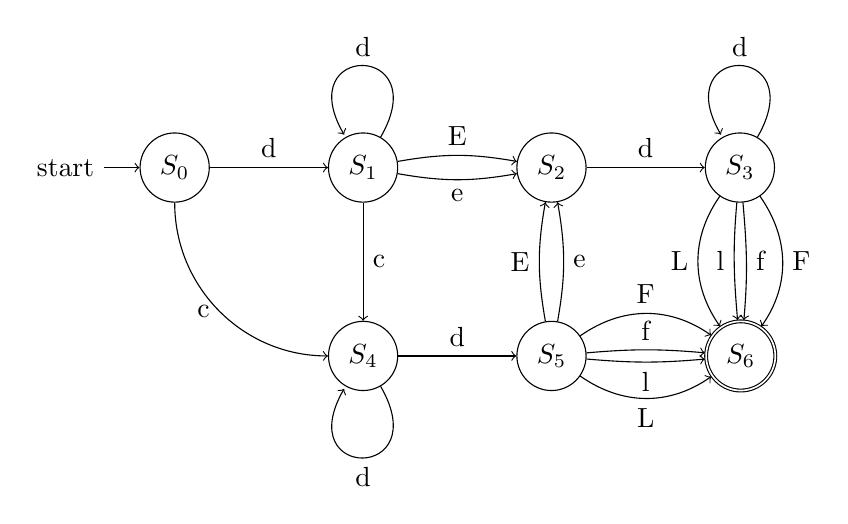
\begin{tikzpicture}[->, auto, node distance=1.5cm]
	\node[state,initial] 	(A)   						{$S_0$}; 
	\node[state] 			(B) [right			=of A] 	{$S_1$}; 
	\node[state] 			(C) [right			=of B] 	{$S_2$};	
	\node[state] 			(D) [right			=of C] 	{$S_3$};
	\node[state] 			(E) [below			=of B] 	{$S_4$};
	\node[state] 			(F) [right			=of E] 	{$S_5$};
	\node[state, accepting]	(G)	[right			=of F]	{$S_6$};	

	\path[->]
	(A) edge 									node 	{d}	(B)
		edge [in=180, out=-90, left]			node	{c}	(E)
	(B)	edge [in=120, out=60, loop, above]		node	{d} (B)
		edge [in=190, out=-10, below]			node	{e} (C)
		edge [in=170, out=10, above]			node	{E} (C)
		edge 									node	{c}	(E)
	(C)	edge 									node	{d}	(D)
	(D)	edge [in=120, out=60, loop, above]		node	{d} (D)
		edge [in=85, out=-85, right]			node	{f}	(G)
		edge [in=55, out=-55, right]			node	{F} (G)
		edge [in=95, out=-95, left]				node	{l} (G)
		edge [in=125, out=-125, left]			node	{L} (G)
	(E)	edge [in=-120, out=-60, loop, below]	node	{d} (E)
		edge 									node	{d}	(F)
	(F)	edge [in=-80, out=80, right]			node	{e}	(C)
		edge [in=-100, out=100]					node	{E} (C)
		edge [in=175, out=5, above]				node	{f} (G)
		edge [in=145, out=35, above]			node 	{F}	(G)
		edge [in=185, out=-5, below]			node	{l} (G)
		edge [in=215, out=-35, below]			node	{L} (G)
;


\end{tikzpicture}
\section*{Code}
\lstset{language=c}
\lstinputlisting{ps1.c}

\end{document} 










